%************************************************
\chapter{Draft}\label{ch:draft}
%************************************************


\section{APDU}

% Reader image, APDU protocol, 

\section{P2ABCE existing code}


In the \ac{P2ABCE} repository \citep{p2abcurl} is available the project's code, divided in two solutions: a complete P2ABCE implementation in Java and a Multos Smartcard implementation as companion for the project.

The Java code is managed by a Maven project, structured using various known design patterns, but not of our interest. The structure we are actually interested in are the REST Services and their use of the Components classes, in which the smartcards are included.

P2ABCE project is based on the concept of smartcards to store the credentials, logical or physical. An interface is defined to communicate with these smartcards, and then different implementations allow to use either \textit{Software Smartcards} or \textit{Hardware Smartcards}. 

The \textit{SoftwareSmartcard} class implements the interface in Java, suitable for tests and self-stored smartcards that any application using P2ABCE may need.

The \textit{HardwareSmartcard} class uses the standard APDU messages [TODO:ref] to interact with smartcards. P2ABCE defines for every method in the mentioned interface, the necessary APDU instructions, and currently relies on \textit{javax.smartcardio} abstract classes (implemented by Oracle in their JRE) to communicate with the smartcard reader. This way, it doesn't matter what manufacturer issues the smartcard, or if it's an Android device, if they support the APDU API, P2ABCE will work with them.

\begin{figure}[bth]
	\begin{center}
		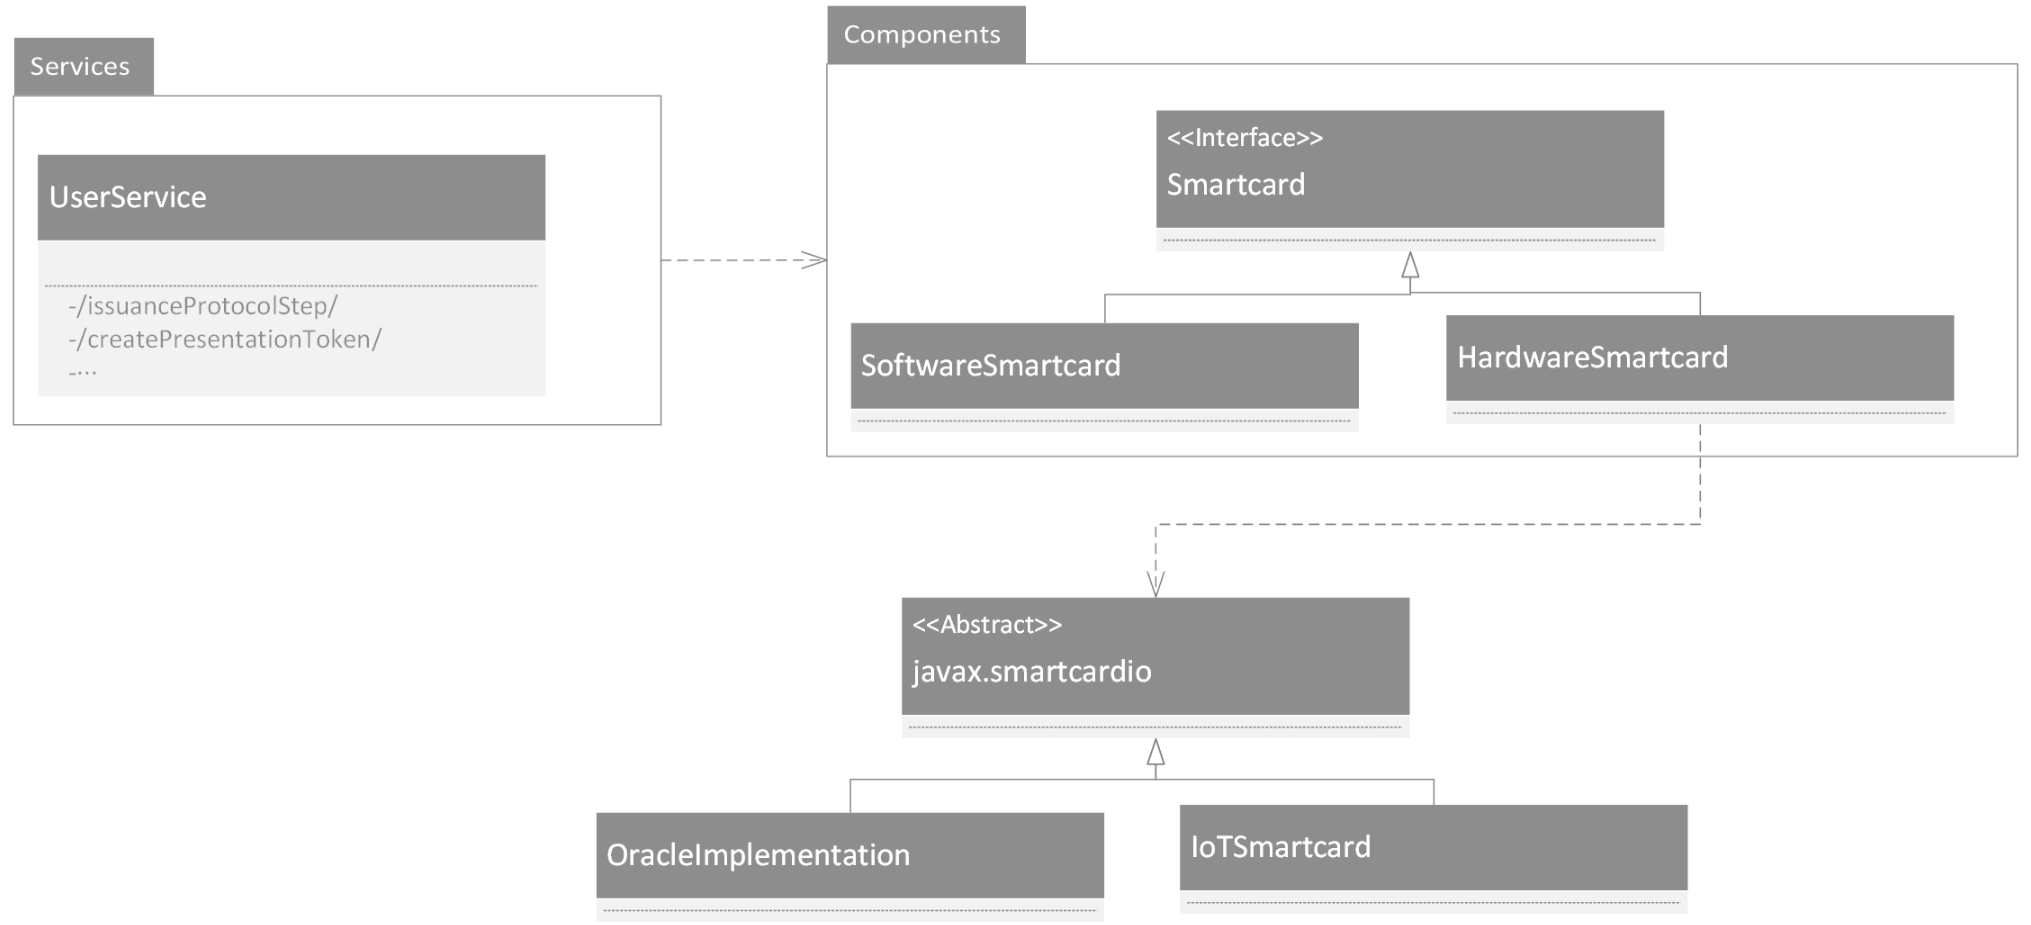
\includegraphics[width=\linewidth]{gfx/p2abceBasicUML}
	\end{center}
	\caption{Basic P2ABCE structure}
	\label{fig:p2abceBasicUML}
\end{figure}


As a PoC the P2ABCE project includes the ABC4Trust Card Lite, an implementation for ML3-36K-R1 Multos Smartcards. The code is written in C, but is very dependent on the Multos framework, aside from numerous bugs and bad coding habits. The code is structured in two files, \textit{main.h} and \textit{main.c}, with 557 and 5157 lines of code respectively. The \textit{main()} function is a 2635 lines long \textit{switch-case} with practically no comments.



At this stage, we have two options to implement our IoT device compatible with P2ABCE:

\begin{itemize}
	\item Implement in C the \textit{Smartcard} interface used by P2ABCE architecture, and using a communication protocol to call the methods from the machine running the P2ABCEngine.
	\item Present the IoT device as a hardware smartcard, using the APDU protocol (already defined, standard and with minimal overload). Providing a \textit{javax.smartcardio} ``IoT implementation'', the already existing \textit{HardwareSmartcard} class can work 
\end{itemize}




\section{Multos}